%%%
%
% $Autor: Wings $
% $Datum: 2021-05-14 $
% $Pfad: GitLab/CornerBLending $
% $Dateiname: Hints
% $Version: 4620 $
%
% !TeX spellcheck = de_DE/GB
%
%%%

\chapter{Manufacturing Hints}

\section{Introduction}

The experimental validation of the monocular visual SLAM (vSLAM) and collision-avoidance pipeline proposed in this thesis relies on a physical mobile robot testbed rather than a purely simulated environment. This chapter documents the hardware platform used throughout the experiments, the manufacturing and assembly considerations that influenced build quality and repeatability, and the design decision to augment the platform with a supplementary mechanical bumper sensor. The purpose of this chapter is twofold: first, to provide a reproducible account of the physical build process so that the platform can be replicated or extended by future work; second, to justify architectural decisions, particularly the bumper integration that preserves the methodological integrity of the thesis's core claim, namely that collision avoidance can be achieved using a \emph{monocular-only} perception stack.

\section{Platform Overview}
The testbed is a SparkFun JetBot v2.1-based differential-drive mobile robot built around the NVIDIA Jetson Nano Developer Kit A02 \cite{NVIDIA:2019, JetsonUserManual:2020}. The platform consists of the following principal subsystems:

\begin{itemize}
	\item \textbf{Compute:} NVIDIA Jetson Nano Developer Kit A02, providing GPU-accelerated inference for the CNN-based collision-avoidance classifier and CPU cycles for the ORB-SLAM2/3-based localization pipeline \cite{NVIDIA:2019}.
	\item \textbf{Perception:} A single front-mounted CSI camera. The Jetson Nano A02 exposes only one CSI camera interface, which is the primary hardware constraint motivating the monocular (rather than stereo or RGB-D) formulation of the SLAM problem in this thesis.
	\item \textbf{Actuation:} A two-motor differential-drive chassis controlled through a Qwiic-interfaced motor driver, communicating with the Jetson Nano over I2C \cite{SparkFun:2019b}.
	\item \textbf{Power:} A single-cell battery pack supplying both the Jetson Nano carrier and the motor driver, imposing a realistic constraint on continuous operating time and peak current draw during simultaneous inference and motor actuation.
\end{itemize}

This configuration positions the platform as a resource-constrained embedded system representative of low-cost indoor service robots \cite{SparkFun:2020}, rather than a laboratory rig with unconstrained compute or power budgets.

\section{Assembly and Manufacturing Considerations}

The chassis and mechanical hardware follow SparkFun's JetBot AI Kit assembly documentation, the most recent published revision of which is the v2.0 guide; this remains functionally applicable to the v2.1 platform used here, as the chassis, motor, and camera mounting geometry are unchanged between revisions \cite{SparkFunJetBotAssembly:2020}. Several manufacturing and assembly considerations proved consequential for build integrity and are recorded here for reproducibility.

\subsection{Motor Orientation and Polarity}

Both DC gearmotors must be installed with their identifying sticker facing outward from the chassis. This orientation is not cosmetic: it determines whether the motor leads map correctly onto the Qwiic Motor Driver's A1/A2 (left channel) and B1/B2 (right channel) terminals \cite{SparkFun:2019b}. An inverted motor produces a robot that yaws or spins rather than tracking a straight commanded trajectory, which would otherwise be misinterpreted as an odometry or control-loop defect during early testing \cite{SparkFunJetBotAssembly:2020}.

\subsection{Standoff Set Confusion}

The chassis kit ships two dimensionally similar sets of brass standoffs --- one for the main chassis frame and a shorter set for the caster ball assembly. Because both sets are packaged together, they are easily interchanged during assembly. Using the wrong set alters the robot's ground clearance and pitch, which in turn shifts the camera's fixed viewing angle relative to the floor plane --- a parameter that matters directly for this thesis, since the collision-avoidance CNN and the ORB feature extractor are both sensitive to the camera's height and tilt relative to the scene \cite{SparkFunJetBotAssembly:2020}.

\subsection{Camera Ribbon Cable Fragility}

The CSI ribbon cable connector on the Jetson Nano is a plastic latch mechanism that degrades with repeated insertion cycles and is not field-replaceable. Given that this thesis's entire perception stack --- both localization and obstacle detection --- depends on a single camera feed, the ribbon cable represents a single point of failure for the whole system. The cable must be inserted with the correct half-twist so that the contact traces align, and re-seating should be minimized once a working configuration is confirmed \cite{SparkFunJetBotAssembly:2020}.

\subsection{Battery Pack Mounting}

In the v2.0 revision, SparkFun relocated the battery mount from the underside of the chassis to the top plate, because the adhesive mounting strip was insufficiently strong to retain the pack underneath during motion \cite{SparkFunJetBotAssembly:2020}. The battery and its leads must be routed to avoid fouling the camera mount or overhanging the rear axle, both of which would alter the robot's center of mass and, consequently, its dynamics during differential-drive maneuvers.

\subsection{Wiring and Tolerance Management}

Motor leads should be routed through the baseplate cutouts before the chassis is closed, and slack should be secured around a standoff rather than left loose near the wheel wells, where it can be caught during rotation \cite{SparkFunJetBotAssembly:2020}. The Jetson Nano's mounting holes are oblong to absorb manufacturing tolerance; standoffs on one side of the board should remain loosely fastened until the board is fully seated, to avoid inducing mechanical stress on the carrier board \cite{JetsonUserManual:2020}.

\section{Design Decision: Auxiliary Bumper Sensor Integration}

\subsection{Rationale}

Although the thesis's central contribution is a monocular vision-based collision-avoidance pipeline, a supplementary mechanical bumper switch was integrated into the platform as an auxiliary safety and evaluation component. This decision is justified on three grounds.

First, \textbf{fail-safe redundancy}. A CNN-based obstacle classifier operating on a single monocular feed is subject to known failure modes, low-illumination frames, textureless or specular surfaces, and objects entering the scene from outside the camera's instantaneous field of view immediately before contact. Vision-based perception in cluttered and dynamic indoor environments remains an open robustness challenge \cite{Cadena:2016, Matthies:2017}, motivating a hardware-level stop signal that is independent of the inference pipeline and therefore immune to these failure modes.

Second, \textbf{resource independence}. The bumper is read as a simple digital GPIO input and does not contend with the shared CSI camera resource used by both the vSLAM and collision-avoidance modules. Given the limited compute and memory budget of lightweight CNN models deployed on resource-constrained edge platforms \cite{zufar:2024}, its inclusion adds redundancy without imposing additional inference or camera-bandwidth load on the perception pipeline.

Third, \textbf{quantitative evaluation utility}. A bumper contact event constitutes an unambiguous ground-truth signal that a physical collision has occurred. Logging bumper triggers alongside the CNN's ``blocked'' predictions enables direct computation of the false-negative rate of the vision-based collision-avoidance classifier is concrete, reproducible metric reported in the results chapter of this thesis.

\subsection{Integration Considerations}

The bumper switch is mounted around the front perimeter of the chassis, positioned to avoid occluding the camera's field of view. It is wired to a Jetson Nano GPIO pin with a pull-up resistor and software debounce logic, triggering an immediate motor-stop interrupt that operates independently of the main perception and control loop \cite{JetsonUserManual:2020}. This ensures that even a stalled or delayed inference cycle does not prevent an emergency stop.

\subsection{Methodological Boundary}

The bumper sensor is explicitly treated as an auxiliary safety and evaluation instrument, not as a component of the core perception architecture under study. This distinction is maintained throughout the thesis to avoid diluting the central research claim --- that indoor obstacle avoidance can be achieved using monocular vision alone \cite{Matthies:2017}, as constrained by the single CSI camera interface of the Jetson Nano Developer Kit A02 \cite{NVIDIA:2019}. All reported collision-avoidance performance metrics are computed from the CNN's vision-based predictions; the bumper is used only for ground-truth verification and as a safety backstop during physical trials, and its activation is reported separately from the vision-only evaluation results.

\section{Mechanical Bumper Design and Integration}
\label{sec:bumper}

While the monocular visual SLAM and CNN-based obstacle-avoidance pipeline described in the preceding chapters provide the robot's primary means of perceiving and reacting to obstacles, both approaches are fundamentally predictive and vision-dependent: they can fail under motion blur, poor lighting, low-texture surfaces, or objects that enter the camera's blind spot close to the chassis. To guard against these failure modes, a purely mechanical, contact-based bumper was designed and fabricated from scratch and integrated directly with the Jetson Nano Developer Kit A02 as a hardware-level, last-resort collision-detection mechanism. This chapter documents the design rationale, physical construction, mounting, electrical integration, and software-level role of this bumper within the overall collision-avoidance pipeline.

\section{Design Rationale}
\label{sec:bumper-rationale}

The SparkFun JetBot v2.1 platform, as configured for this thesis, does not include an inertial measurement unit (IMU), wheel encoders, or any dedicated proximity sensor (e.g., ultrasonic or infrared rangefinders). Consequently, the only sources of environmental information available to the robot are the single front-facing monocular camera feed, which is shared between the vSLAM localization module and the CNN-based obstacle-detection module. Since both of these modules operate on the same visual stream and both are susceptible to correlated failure modes (e.g., sudden illumination changes, featureless walls, or fast-approaching obstacles at close range where perspective cues collapse), a physically independent, sensor-diverse fallback was considered necessary to prevent hard collisions that could damage the chassis, the camera mount, or the motor drivetrain.

\begin{figure}[H]
	\centering
	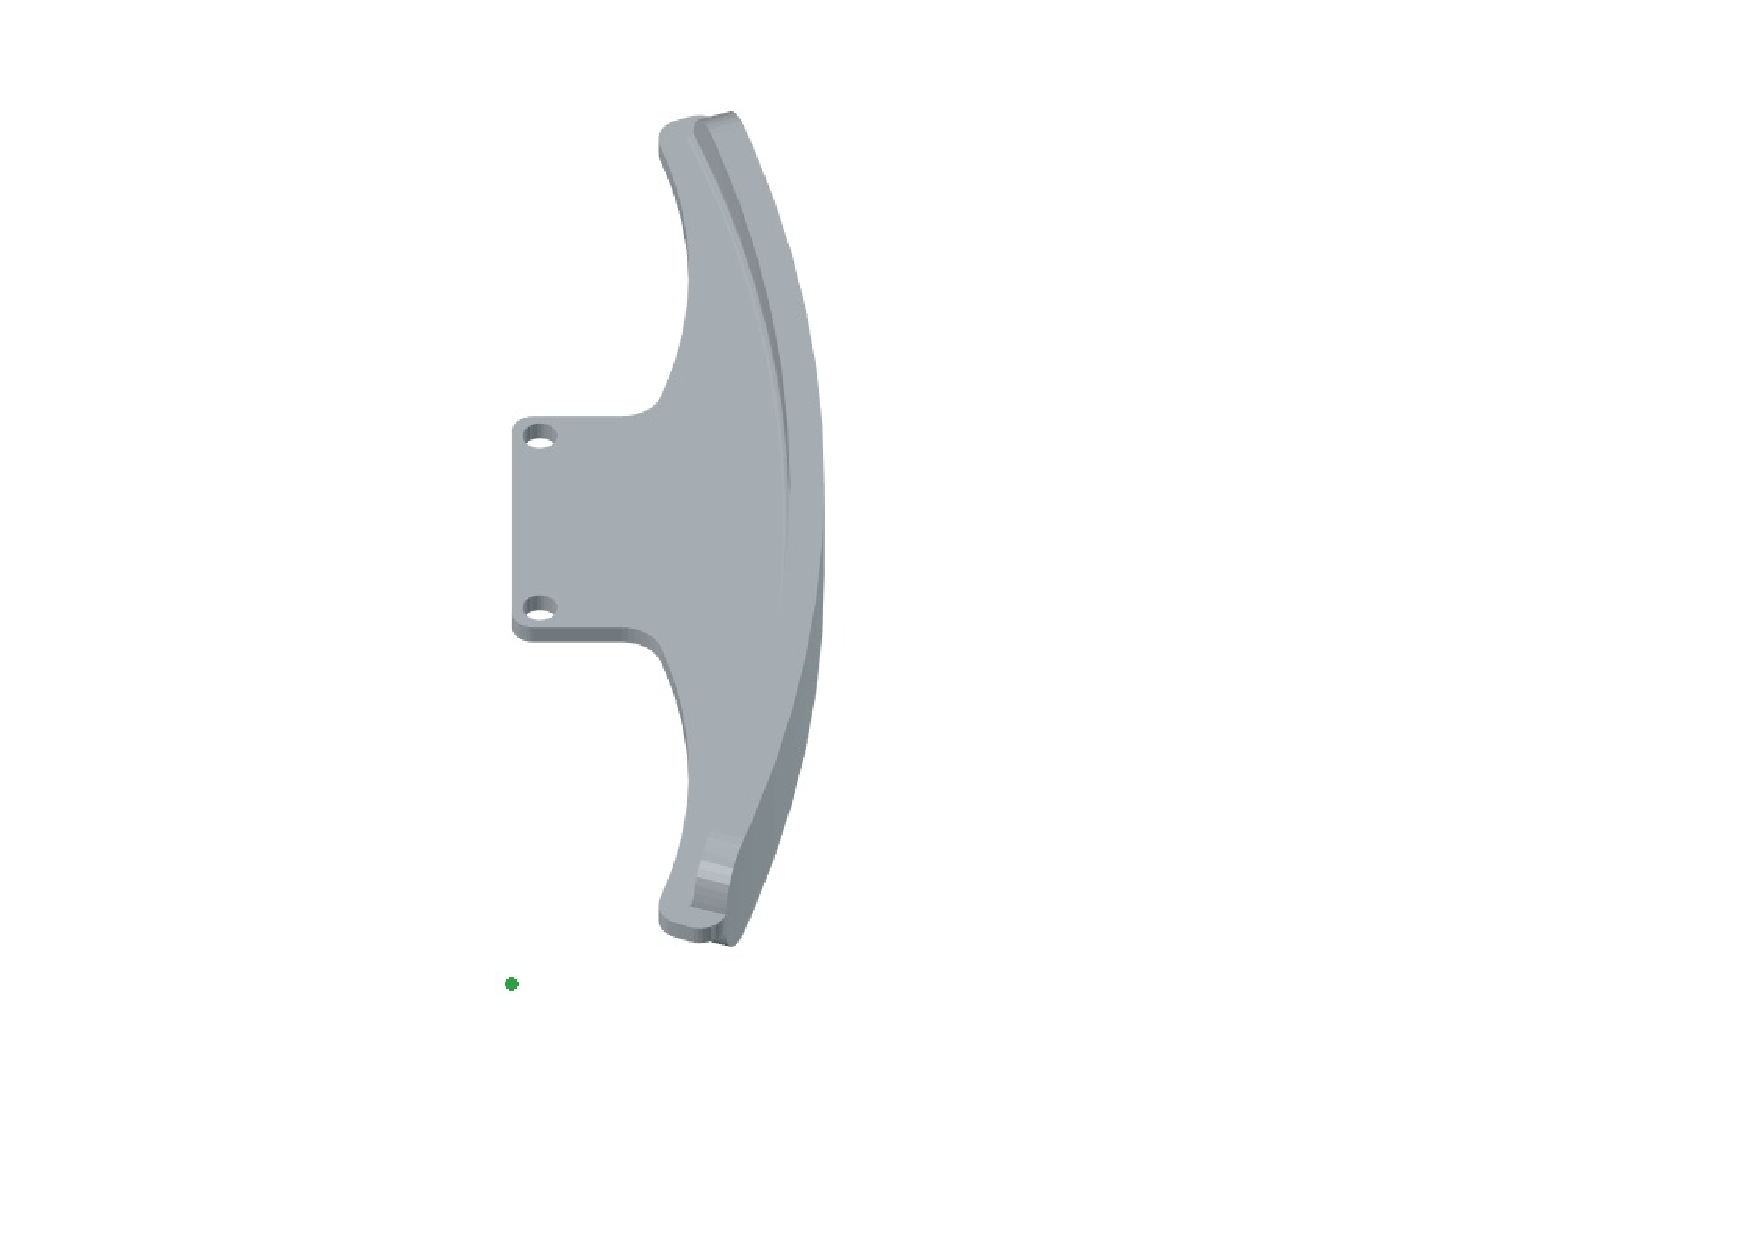
\includegraphics[width=0.7\linewidth]{Images/MobileRobotBumper}
	\caption{Bumper for Mobile Robot}
	\label{fig:mobilerobotbumper}
\end{figure}


A mechanical, switch-based bumper was chosen over an additional active sensor (such as an ultrasonic or infrared ranger) for three reasons. First, it requires no additional calibration or software filtering, since it produces a binary contact signal that is trivial to interpret. Second, it consumes negligible power and computational resources, which is important given the constrained power budget of the single-cell battery pack. Third, it is entirely independent of lighting conditions and surface texture, making it complementary rather than redundant with respect to the vision-based pipeline.

\section{Materials and Construction}
\label{sec:bumper-materials}

The bumper structure was assembled entirely from off-the-shelf and 3D-printed components, with no pre-made bumper kit used. The main structural element is a semi-circular ring fabricated from polylactic acid filament using fused deposition modeling (FDM) 3D printing, chosen for its rigidity, ease of printing, and low weight relative to the JetBot chassis. The ring was designed to wrap around the front half of the chassis perimeter, covering the region most likely to make first contact with obstacles given the robot's differential-drive kinematics and forward-biased camera field of view.

Two miniature tactile lever-arm microswitches were embedded at the leading edge of the bumper ring, spaced symmetrically about the chassis centerline to allow the system to distinguish between a left-side, right-side, or head-on collision based on which switch (or both) is triggered. A thin compliant foam strip was affixed along the outer edge of the printed ring to absorb minor impacts, provide a small amount of pre-travel before the microswitches engage, and reduce the shock transmitted to the printed structure itself.

\section{Mounting on the Chassis}
\label{sec:bumper-mounting}

The bumper assembly is mounted at the front of the JetBot chassis, ahead of and below the camera mount, so that it does not obstruct the monocular camera's field of view while still providing forward impact protection. The printed ring is secured to the existing chassis standoff holes using M3 nylon screws and standoffs, chosen to keep the added mass low and to avoid interfering with the Qwiic motor controller and wiring harness located on the chassis underside. This mounting position was selected after considering the robot's turning behavior: because the differential-drive base can pivot in place, the bumper's semi-circular coverage ensures that both frontal and near-frontal oblique collisions are detected regardless of the robot's instantaneous heading during an avoidance maneuver.

\section{Electrical Integration}
\label{sec:bumper-electrical}

Each microswitch is wired as a simple normally-open contact switch, pulled high through an internal pull-up configuration and connected directly to a dedicated GPIO pin on the Jetson Nano Developer Kit A02's 40-pin expansion header. This keeps the bumper entirely independent of the Qwiic I2C bus used for the motor controller, so that a bumper-triggered event can be read and acted upon even if the I2C bus is congested or temporarily unresponsive. When a switch closes on contact, the corresponding GPIO line is pulled low, generating a signal that is polled by a lightweight background thread on the Jetson Nano.

No additional signal conditioning circuitry was required beyond basic debouncing, which is handled in software (Section~\ref{sec:bumper-software}) rather than with discrete RC filtering hardware, in order to keep the electrical design as simple and failure-resistant as possible.

\section{Software Integration with the Collision-Avoidance Pipeline}
\label{sec:bumper-software}

At the software level, the bumper is treated as a hard interrupt source with the highest priority in the overall collision-avoidance stack. A dedicated GPIO polling routine, running independently of the vSLAM and CNN inference threads, continuously monitors both microswitch lines at a fixed sampling rate and applies a short software debounce window to filter out spurious transitions caused by vibration during normal driving.

Whenever a bumper contact event is confirmed, the routine immediately issues a motor-stop command directly to the Qwiic motor controller, pre-empting any velocity command currently being issued by the CNN-based obstacle-avoidance policy or the vSLAM-driven navigation logic. Following a stop, the robot executes a short pre-programmed reverse-and-turn maneuver away from the side on which contact was detected (left switch, right switch, or both, in the head-on case) before control is returned to the primary vision-based pipeline. This ensures that the mechanical bumper functions strictly as a safety net beneath the monocular vSLAM and CNN-based obstacle-avoidance system, intervening only when the vision-based pipeline has already failed to prevent a physical collision.

